\documentclass[border=3pt,tikz]{standalone}
\usepackage{amsmath}
\usetikzlibrary{calc}
\usetikzlibrary{arrows.meta} % for arrow size
\begin{document}
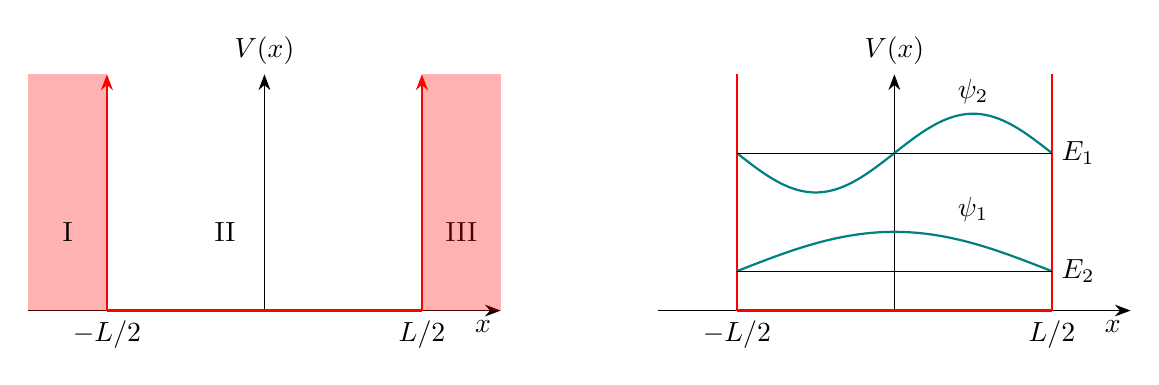
\begin{tikzpicture}[scale=1]


    \draw[, -{Stealth[length=2mm]}] (0, 0) -- (0, 3) node [above] {$V(x)$};
    \draw[, -{Stealth[length=2mm]}] (-3, 0) -- (3, 0) node [below left] {$x$};
    \draw[red, thick, -{Stealth[length=2mm]}] (-2, 0) -- (-2, 3);
    \draw[red, thick, -{Stealth[length=2mm]}] (2, 0) -- (2, 3);
    \draw[red, thick] (-2, 0) -- (2, 0);
    \node[below] at (-2, 0) {$-L/2$};
    \node[below] at (2, 0) {$L/2$};
    
    \fill [fill=red,fill opacity=0.3] (-2,0) rectangle (-3,3);
    \node[] at (-2.5, 1) {$\rm{I}$};
    \node[] at (-0.5, 1) {$\rm{II}$};
    \node[] at (2.5, 1) {$\rm{III}$};
    
    \fill [fill=red,fill opacity=0.3] (2,0) rectangle (3,3);
    
    \begin{scope}[shift={(8,0)}]
    \draw[, -{Stealth[length=2mm]}] (0, 0) -- (0, 3) node [above, scale=1] {$V(x)$};
    \draw[, -{Stealth[length=2mm]}] (-3, 0) -- (3, 0) node [below left] {$x$};
    \draw[red, thick] (-2, 0) -- (-2, 3);
    \draw[red, thick] (2, 0) -- (2, 3);
    \draw[red, thick] (-2, 0) -- (2, 0);
    \node[below] at (-2, 0) {$-L/2$};
    \node[below] at (2, 0) {$L/2$};
    
    
    \draw[teal, thick] plot[variable=\t,domain=-2:2, samples=100, smooth,thick] ({\t}, { 0.5*cos( \t * 45) + 0.5});
    \draw[] (-2, 0.5) -- (2, 0.5) node [right] {$E_2$};
    \node[above] at (1.0, 1.0) {$\psi_1$};
    
    
    \draw[teal, thick] plot[variable=\t,domain=-2:2, samples=100, smooth,thick] ({\t}, { 0.5*sin( \t * 90) + 2});
    \draw[] (-2, 2) -- (2, 2) node [right] {$E_1$};
    \node[above] at (1.0, 2.5) {$\psi_2$};
    
    \end{scope}
    \end{tikzpicture}
\end{document}